% !TeX root = ../main.tex
% Add the above to each chapter to make compiling the PDF easier in some editors.

\chapter{Building Flows in Weight-Space}\label{chapter:method}

\begin{figure}[h!]
    \centering
    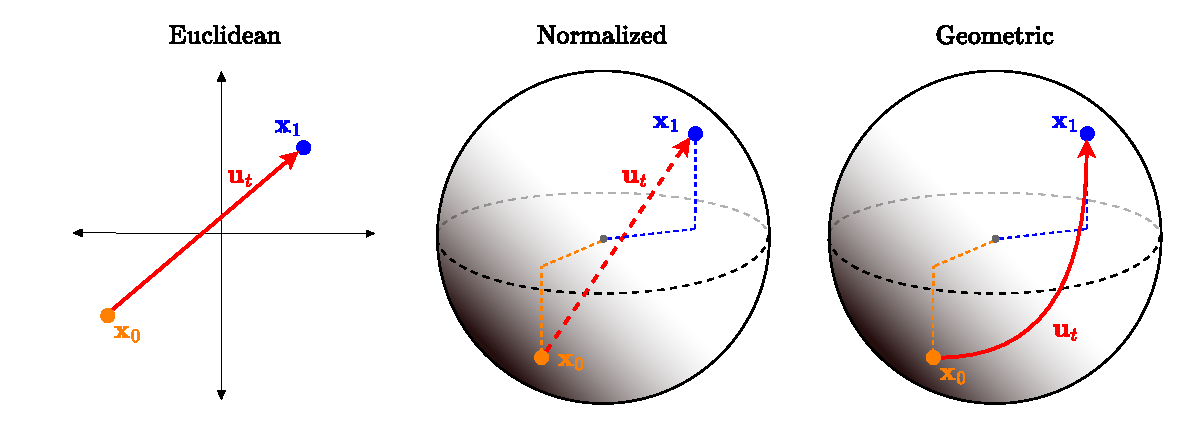
\includegraphics[width=\textwidth]{figures/flow_types.drawio.pdf}
    \caption{\label{fig:flow_types} Flow Types}
\end{figure}

Some more text 

\begin{figure}[h!]
    \centering
    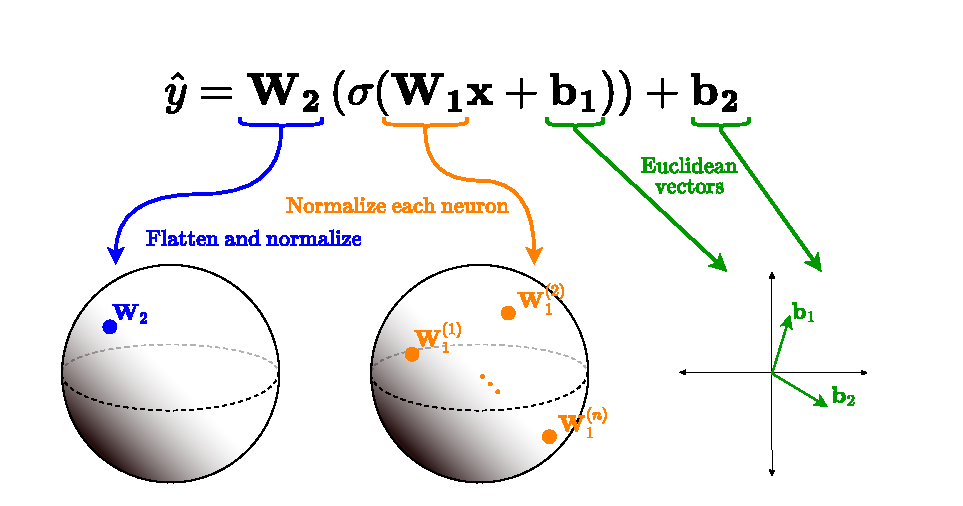
\includegraphics[width=\textwidth]{figures/canonicalization.drawio.pdf}
    \caption{\label{fig:canonicalization} Canonicalization}
\end{figure}

Some text 